%\documentstyle{article}  % by default 10pt
\documentclass{article}  % by default 10pt

\usepackage{graphicx}
\usepackage{amsfonts}
\usepackage{subfigure}
\usepackage{times}
\usepackage{cite}
\usepackage{subfigure}
\usepackage{amsmath}
\usepackage{amssymb}
\usepackage{url}
\usepackage{tikz}
\usepackage{verbatim}
\usepackage{array}
\usepackage{wrapfig}

%
% Page dimensions.
%
\oddsidemargin  -0.2in % 
\evensidemargin -0.2in %
\topmargin      -1.00in % (adjusted for printer bias)
\headheight      .00in  % (no headers)
\headsep         .75in  % (top margin + headers + skip)
%\footheight     12.0pt  % ??? (seems to work ok)
\footskip       75.0pt  % ??? ( "   "  )
\textheight     9.425in % (instructions: 9 1/8" min, 9 7/16" max)
\textwidth      6.7in   %
%\linespread{0.9}
%
  % Paragraph changes.
  %

  \parindent=10pt
  %\parskip=10pt
  %


  \def\@maketitle{\vbox to 2.6in{\hsize\textwidth
    \linewidth\hsize \vfil \centering
    {\large \@title \par}
    \vskip 2em
    {\normalsize
      \begin{tabular}[t]{c}\@author
	\end{tabular}\par}
      \vfil}
  }


\begin{document}

\title{Integrated Modeling of Performance, Power and Resilience for Adaptive Parallelism}

\author{Dong Li$^{\dag}$, Edgar Leon$^{\star}$, and Bronis de Supinski$^{\star}$ \\
    $^{\dag}$Oak Ridge National Laboratory and $^{\star}$Lawrence Livermore National Laboratory \\
    lid1@ornl.gov (main contact), \{leon, bronis\}@llnl.gov	\\
}

\date{}

\maketitle

\noindent {\Large \textbf{Motivation}}   \\
The path to exascale presents increased parallelism to reach performance targets with constrained power consumption.
Meanwhile, efforts to reduce power and increase component counts may lead to significant increase in the number of faults,
making system resilience a grand challenge for exascale systems. To address challenges of 
performance, power, and resilience (PPR), modeling methods must evolve and consider
them in concert. Furthermore, modeling methods must be rapid and accurate, such that
runtime can effectively enable dynamic evaluation of tradeoffs between PPR.

The common practice of current modeling methods employs analytical models or architectural simulators to study PPR.
The investigations of performance, power, and resilience are isolated based on individual modeling infrastructures
and methodologies.
Furthermore, many modeling tools and techniques are heavyweight, and cannot be easily employed at runtime.
As a result, we do not have any efficient modeling mechanism that directs runtime management 
and allows us to explore the optimal operating point in the 3D search space of PPR.

In this position paper, we study modeling of PPR based on an integrated %uniform 
modeling infrastructure. 
The infrastructure collects utilization information from 
a common set of hardware components to characterize applications and predict PPR.
We study our modeling techniques in the context of runtime parallelism management for the OpenMP
programming model.
The management and optimization of parallelism is fundamental to meet PPR requirements
of exascale systems.
Scientific applications typically have inherent parallelism that varies across execution phases~\cite{nvram_ipdps12}.
Matching the degree of parallelism (named \textit{parallelism configuration} in the rest of paper) between application and hardware
have complicated implications on PPR~\cite{mpiopenmp_ipdps10, mpiopenmp_tpds13, dsn_pact08, dsn_ics06}. 
We aim to use a model-driven approach to decide optimal parallelism based on user-defined policies
and enable adaptive parallelism at runtime.

%Relative order; no absoultely requirement on accuracy.
%The path to exascale presents increased parallelism with billions of concurrently-executing threads 
%at the intra-node and inter-node levels. 
%The management and optimization of parallelism is fundamental to meet performance, 
%energy-efficiency and resilience requirements
%of systems and applications at exascale.

\vspace{10pt}

\noindent {\Large \textbf{Our Position}}  \\
Our modeling methodology is based on two observations.
First, performance, power, and resilience have first-order or second-order correlation with hardware components utilization.
From performance perspective, our work reveals that counting number of accesses to memory hierarchy and counting total
number of instructions can serve as a strong indicator to performance with various parallelism~\cite{mpiopenmp_tpds13, mpiopenmp_ipdps10, dct_pmbs11, dct_iiswc12}.
From power perspective, power consumption is related with hardware access intensity, 
shown in previous work~\cite{mpiopenmp_tpds13, powermodel_sigmetrics03, powermodel_micro03}.
From resilience perspective, resilience is related with both application execution time ($t$) 
and number of hardware accesses ($\#HA$).
Given hardware failure rates for specific hardware components, a longer application execution time and a larger number of hardware accesses
indicate that the application is more exposed to random occurrences of hardware failure events (including both hard and soft errors).
We introduce a new metric, named as \textit{vulnerability factor} (VF) and defined as $VF = t*\#HA$,
to quantify application vulnerability. Based on this metric, resilience is also related with hardware component utilization as performance and power is. 
 
Second, given a specific parallel region, PPR for different degree of thread-level parallelism have strong statistical correlation.
Hence, based on information of hardware components utilization
collected from a few samples of parallelism configurations, %(each of which employs a specific number of OpenMP threads), 
we can make PPR prediction for other parallelism configurations. 
We call those representative samples, \textit{seminal configurations}.

Based on the above two observations, the PPR model construction 
includes two phases: offline model training and online model selection.
During offline model training, we use a machine learning-based approach
to decide which hardware components utilization information is
mostly correlated with PPR. 
The information should be measurable with lightweight hardware counters.
Furthermore, we choose seminal configurations based on an empirical observation.
The empirical observation reveals that PPR data with different degree of parallelims
can be visually clustered into different groups. The parallelism configuration
which is the closest to the center of each group is chosen as a 
seminal configuration. We build a series of PPR models to
capture diverse hardware features and application characteristics during offline training.
During online model selection, we use a few sample iterations in OpenMP parallel regions to execute
wtih seminal configurations and collect hardware components utilization
information, based on which we decide which model should be employed.

Based on the above modeling methodology, runtime can predict PPR for any untested 
%thread-level 
parallelism configuration. Built on top of the models,
runtime chooses the best parallelism for each OpenMP parallel region based 
on high-level user-defined policies, for example, minimizing VF without performance and power
loss, or minimizing the multiplication of time, power, and VF to achieve
an optimal tradeoff of PPR, or achieving the best performance and resilience within a power cap.
We have established the model infrastructure to predict performance and power on many-core platforms.
We plan to extend the modeling methodology to better capture effects of
data layout and memory-level parallelism on PPR.
We also plan to extend the models to support PPR prediction 
and parallelism scheduling on
heteroegenous platforms. 
Figure~\ref{fig:general_framework} generally depicts the framework
for model construction and deployment.
%to be a new layer between OpenMP directives,

\begin{wrapfigure}{r}{0.4\textwidth}
\begin{center}
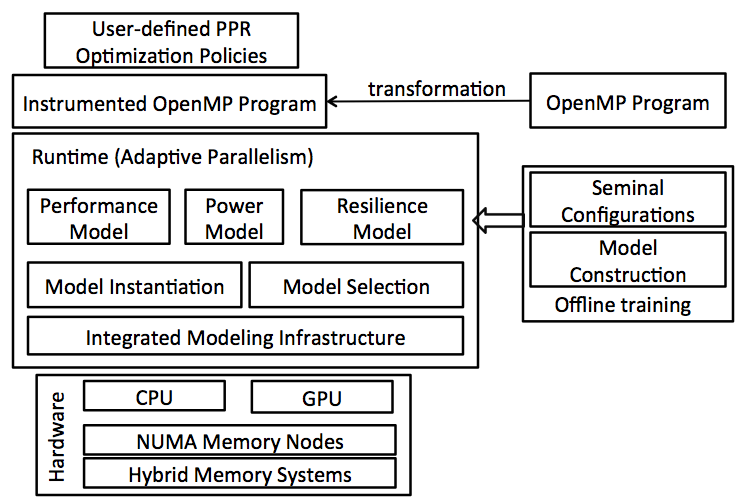
\includegraphics[width=0.39\textwidth]{figures/general_framework.png}
\end{center}
\caption{The general framework for adaptive parallelism with integrated PPR modeling}
\label{fig:general_framework}
\end{wrapfigure}

\vspace{10pt}

\noindent {\Large \textbf{Related Work}}   \\
Performance, power, and resilience modeling and simulation have been studied before, but mostly with
an isolated approach. Some of the works employ analytical models or empirical models
to achieve joint optimization of power and performance, 
for example green queue~\cite{sdscpower_hppac12, sdscpower_ccpe12, sdscpower_cgc12}, 
Adagio~\cite{rountree_sc07, rountree_ics09}, and workload consolidation~\cite{taskconsolidation_ipdps10, gpusolidation_srmpds11}.
Some of the work use detailed hardware analysis for hardware-oriented resilience modeling. 
For example, Mukherjee et al.~\cite{avf_micro03} define an architectural vulnerability factor
(AVF) as the probability that a fault in a particular structure will result an error. Biswas et al.~\cite{avf_isca05} show how to compute the
AVF of address-based processor structures based on a detailed analysis of architecturally correct execution.
Sridharan and Kaeli~\cite{pvf_selse10, pvf_hpca09} introduce a new metric to capture the architecture-level fault masking inherent in a
program. Furthermore, fault injection has also been widely used to understand application vulnerability in 
~\cite{li:2012:classifying, multigrid_ics12, fj_asplos12, fj_dns12, lanl_fi_europar11}.
\vspace{10pt}

\noindent {\Large \textbf{Assessment}}   \\
\textbf{Challenges addressed:} 
Exascale systems demand modeling and simulation capabilities to achieve joint optimization of 
performance, power, and resilience. Furthermore, modeling and simulation infrastructures should
provide rapid and dynamic evaluation of tradeoff between PPR. Our modeling infrastructure is extremely
valuable for runtime management of system resource (e.g., thread-level parallelism and  
memory-level parallelism in our case).
%The proposed approach addresses resilience and power challenges for future exascale systems as

\textbf{Maturity:} 
Performance, power and resilience modeling and simulation have been separatrely considered in the
existing work (see related work).
Also, we have established preliminary capabilities to model performance and power for OpenMP parallel 
regions with various parallel configurations. Our modeling infrastructure brings ignorable 
performance overhead while providing great energy saving for DOE applications with 
the hybrid MPI/OpenMP programming model.
However, our current modeling infrastructure is only a start and
requires significant new work to improve modeling infrastructure
especially for resilience modeling and heterogeneous platform. 
%The proposed idea builds on successful research, including the DOE funded Blackcomb 

\textbf{Uniqueness:}
Our modeling methodology is tightly coupled with the OpenMP programming model,
and aims to reveal PPR difference between different parallelism configurations.
Unlike prior work that focuses on accurate prediction,
our work focuses on coarse-grained PPR indicator to guide runtime management.

\textbf{Novelty:} 
Our modeling methodology reveals statistical correlation
between measurable hardware events, application characteristics and 
PPR. The unique set of features and opportunities provided by our models
provide fast exploration of PPR to achieve multi-dimensional optimization.     

\textbf{Applicability:} 
The proposed PPR models have been deployed in OpenMP runtime to
optimize performance and energy efficiency.  
The proposed models work as a critical step to implement adaptive parallelism,
and provide a new approach for massive parallelism management.

\textbf{Effort:} We need to add new features into the current modeling infrastructure,
including resilience modeling and memory-level parallelism modeling,
and interoperating with other ModSim tools.
To provide a broad coverage of system properties and resources, we need
a significant effort contributing to an agile and integrated modeling
of PPR.

\bibliography{li}
\bibliographystyle{plain}

\end{document}
